\section{Thursday, March 21st: Stochastic Processes}
\subsection{Logistics}
\begin{enumerate}
    \item Peer Review -- due Today.
    \item Optional Reading posted -- T\&C 4, \underline{GP notes}.
    \item \underline{Enjoy Spring Break!}
\end{enumerate}

\subsection{Goals}
\begin{itemize}
    \item ($\cdot$) Processes
    \item ($\cdot$) \underline{Entropy Rates}
\end{itemize}

\subsection{Stochastic Process}
\begin{shaded}
A \textbf{stochastic process} $\{X_j\}_{j=1}^{\cdots}$ or $\{X(t)\}_{t}$ is indexed by ``time'', and is discrete or continuous.
\end{shaded}

\subsubsection{Joint distribution over a countable random vector}
There will be a joint distribution for any subset ($\{X_j\}_{j\in\mathcal{J}}$ or $\{X_j\}_{j\in\mathcal{J}}$) of variables, we have:
\begin{equation}
    \P(X_1=x_1,X_2=x_2, \ldots, X_n=x_n)
\end{equation}

There is no notion of 0 time -- it's arbitrary.

\subsubsection{Stationary of a Process}
\begin{shaded}
A process is \textbf{stationary} if $p(\{X_j\}_{j\in\mathcal{J}}=\{x_j\})=p(\{X_{j+s}\}_{j\in\cJ} = \{x_j\})$, if any set of samples is unchanged under time translation.
\end{shaded}

\subsubsection{Stationary Distribution}
\begin{shaded}
If a process, $\{X_j\}_{j=1}^{\cdots}$, is stationary then the corresponding Stationary Distribution is: 
\begin{equation}
p_{\text{stat}}(x) = P(X_j = x) \text{ for any $j$}
\end{equation}
\end{shaded}

\subsubsection{Ergodicity of Stochastic Processes}
\begin{shaded}
If a process, $\{X_j\}_{j=1}^{\cdots}$, is stationary then it is also \underline{Ergodic}: 
\begin{equation}
\label{ergodic-stat}
\E_{X\sim p_{\text{stat}}}[f(X)] = \Bar{f}_{\text{stat}}
\end{equation}

\begin{equation}
\label{ergodic-time}
\frac1n \sum_{j=1}^n f(X_j) = \Bar{f}_{\text{time}}(n) \stackrel{\small{n\to\infty}}{\to} \Bar{f}_{\text{time}}
\end{equation}
We expect the long-term avg to be concentrated and to converge.

The fact that \eqref{ergodic-stat} and \eqref{ergodic-time} are the same, $\Bar{f}_{\text{stat}}=\Bar{f}_{\text{time}}$, is what makes us ergodic.
\end{shaded}

\subsection{Markov Process}
A random process whose future probabilities are determined by its most recent values. A stochastic process $X(t)$ is called Markov \\
if $X(t+s),\quad s>0$ is conditionally $\indep$ of $X(t-h),\quad h>0$ given $X(t)$.
\begin{shaded}
The future is conditionally independent of the past given the present.
\end{shaded}

\begin{equation}
\operatorname{Pr}\left(X_{n+1}=x_{n+1} \mid \underbrace{X^{(n)}}_{
X_{n}, X_{n-1}, \ldots X_1}=x^{(n)}\right)
=
\underbrace{P\left(X_{n+1}=x_{n+1} \mid X_{n}=x_n\right)}_{\text{Transition prob.: } 
P_{i, j}^{\blue{(n)}}=P\left(X_{n+1}=i \mid X_n=j\right)}
\end{equation}

\subsubsection{Time Autonomous}
\begin{equation}
\Pr\left(X_{n+i}=i \mid X_{n}=j\right)=\Pr\left(X_2=i\mid X_1=j\right) 
\quad
\forall{i, j} \text { and } n. 
\end{equation}

\subsection{Transition Matrix}
The matrix $P$ has entries $P_{i, j}$ which give you the probability of going from $j$ at the present to $i$ in the future. That is, $P_{i,j}=\Pr(X_{n+1}=i\mid X_n=j), \quad P =\begin{bmatrix}
    \mid & \mid & & \mid \\
    p_1 & p_2 & \ldots & p_{|\cX|} \\
    \mid & \mid & & \mid
\end{bmatrix}$
with the $j$th column being the conditional distribution of the future given the present.

\begin{important}
Note that we use the following convention: this matrix is column-stochastic.
\end{important}

\begin{equation}
    \Pr(X^{(n)} = x^{(n)}) = 
    \underbrace{\left(
    \prod_{j=1}^n \P_{X_{j+1} X_j}
    \right)}_{\Pr(X^{(n)} = x^{(n)} \mid X_1=x_1)}
    p(X_1=x_1)
\end{equation}
where $p(X_1=x_1)$ is the initial distribution for the probability of where I start.

\subsection{Irreducibility}
A discrete-time, discrete-state MC is \underline{irreducibile} if
$\forall x_1=i, x_n=j \quad\exists$ a path $x^{(n)} = \{i, \ldots, j\}\st P(X^{(n)} - x^{(n)} \mid X_1 = i)>0$.

\subsection{Aperiodic}
A discrete-time, discrete-state MC is \underline{aperiodic} if
it's period is 1.

\subsubsection{Period}
A Period of the process is its GCD of the length of all cycles:
$$x^{(n)}  = \{x_1,x_2,\ldots, x_1\},\quad  P(X_n=x_n \mid X_1 = x_1)>0$$

\begin{figure}[H]
    \centering
    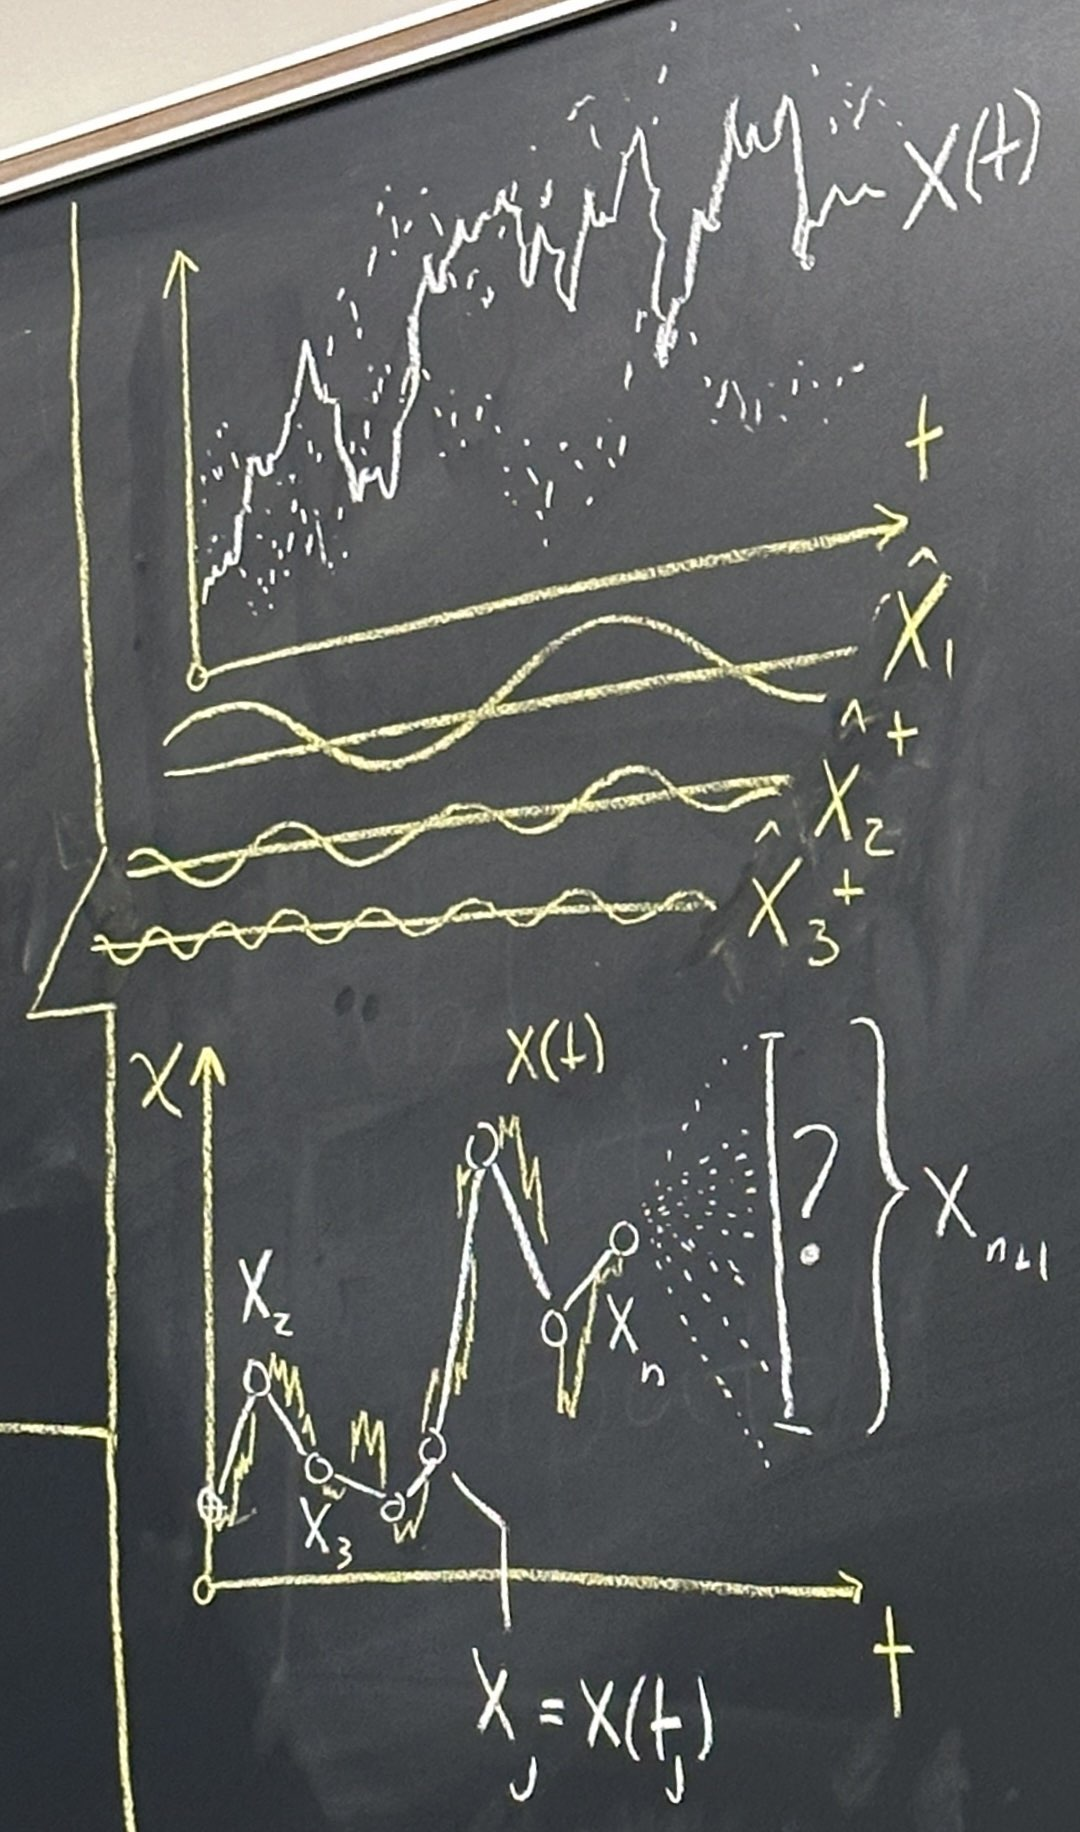
\includegraphics[height=25pc,width=40pc]{lectures/wk10/img/lec19_sp.jpeg}
    \caption{Various periods of Stochastic Processes}
    \label{fig:stoch-procs}
\end{figure}

\subsection{Perron-Frobenius Theorem}
If $P$ is column-wise Stochastic (transition for a $d-t, d-s$ MC) that is \underline{irreducible} \& \underline{aperiodic} then:

it converges to a \underline{unique stationary} distribution from any initial distribution, is stationary if initialized with $P_{\text{stat}}$, is \underline{ergodic}.


\begin{enumerate}
    \item $\exists$ a simple (A simple eigenvalue is an eigenvalue with multiplicity one -- the eigenvalue is unique) largest (in magnitude) eigenvalue $\lambda_{\max}(P)\in\R^+$.
    \item It's corresponding eigenvector $v_{\max}(P)\quad v_{\max}(x) \geq 0$ ($v \in \R^{+|\cX|})$
\end{enumerate}


Tldr;\\
A real square matrix with positive entries has a unique eigenvalue of largest magnitude and that eigenvalue is real ($\lambda\in\R$).

\subsection{Gershgorin Disk Theorem}
If $A\in \C^{n\times n}$ (or for simplicity, we will just provide a proof for $A\in \R^{n\times n}$), then $\lambda_j(A)\in \cup_{j=1}^n D(a_{jj}, \sum_{i\neq j} |a_i|)$

$
\sum_{i\neq j} |p_{ij}| = \sum_{i\neq j} p_{ij} = 1 - p_{jj}
$

This gives us that $|\lambda_j(P)|\leq1$.

$\therefore\quad \lambda_{\max}(P)=1$

$|\lambda_j(P)|=1\quad$ (if $j\geq2$).

\hrulefill

\begin{algorithm}
\caption{Algorithm for $p_0: p_n\stackrel{n\to\infty}\to \R$}
\begin{algorithmic}
\State \textbf{Initialize: } $\Pr(X_0=x)=p_0$.
\State \textbf{Find: } $p_n^{(x_n)}=\Pr(X_n=x_n)=\displaystyle\sum_{x_{n-1}}
\underbrace{\Pr(X_n=x_n\mid X_{n-1}=x_{n-1})}_{P_{x_n, x_{n-1}}} \underbrace{\Pr(X_{n-1}=x_{n-1})}_{P_{n-1}^{(x_{n-1})}}$
\Ensure Matrix columns add to 1.
\While{stopping criteria not met}
\State $p_n \gets Pp_{n-1}$
\State $p_n \gets P^n p_{0} = V\Lambda^{n} VV^\top p_0=V_{\max}(VV_{\max}^\top p_0)+\cO(\lambda_2^n)
= V_{\max}(\underbrace{\mathbbm{1}^\top p_0}_1)+\cO(\lambda_2^n)
= V_{\max}+\cO(\lambda_2^n)
$
\EndWhile
\State \Return $p_n$
\end{algorithmic}
\end{algorithm}

\subsection{Entropy Rate}
% pls help





Define $H'[\cX]=\displaystyle\lim_{n\to\infty} H[X_n \mid X^{(n-1)}]$.
\begin{enumerate}
    \item If the process is stationary then the sequence $H[X_n\mid X^{(n-1)}]$ is non-increasing and converges.
    \begin{shaded}
        \begin{proof}
        Undoing a conditioning should increase entropy:
            \begin{align*}
                H[X_n\mid X^{(n-1)}] 
                &=
                H[X_n \mid X_{n-1}, X_{n-2},\ldots,X_{2},X_{1}]
                \\
                &\leq H[X_n \mid X_{n-1}, X_{n-2},\ldots,X_{2}]
                \\
                &= H[X_{n-1} \mid X_{n-2}, X_{n-3},\ldots,X_{1}]
                &&[\text{Invariant under time shifts}]
                \\
                &= H[X_{n-1}\mid X^{(n-2)}]
                \\
                \underbrace{H[X_n\mid X^{(n-1)}]}_{>0}
                &\leq H[X_{n-1}\mid X^{(n-2)}]
                &&[\text{non-incr seq + bounded below $\implies$ conv.}]
            \end{align*}
        \end{proof}
    \end{shaded}
    \item The limit of the new entropy (the cndtl entropy in the future given the past) is $H[\cX]=H'[\cX]$.
    \begin{shaded}
        \begin{proof}
            \begin{align*}
                H[\cX] 
                &=
                \lim_{n\to\infty}\frac1n H[X^{(n)}] 
                = \lim_{n\to\infty} (\frac1n\sum_{j=1}^n H[X_j\mid X^{(j-1)}])
                \to H'[X]
            \end{align*}
        \end{proof}
    This can also be understood (the difference between the observed value of a variable at time $t$ and the optimal forecast of that value based on information available prior to time $t$) the innovation.
    \end{shaded}
\end{enumerate}
